% !TEX root = ../../buch.tex
% !TEX encoding = UTF-8
%
\section{Die Taylor-Reihe als Grundlage}
\label{pade:section:taylor}
\kopfrechts{Taylor-Reihe}

Die Padé-Approximation baut vollständig auf der Taylor-Reihe einer Funktion auf. Ohne die Taylor-Reihe lässt sich keine Padé-Approximation konstruieren, da sämtliche Koeffizienten der späteren rationalen Funktion aus den Koeffizienten der Taylor-Reihe bestimmt werden. Bevor das eigentliche Verfahren vorgestellt wird, sollen deshalb zunächst die wichtigsten Eigenschaften der Taylor-Reihe erläutert werden.

Die Grundidee der Taylor-Reihe besteht darin, eine genügend oft differenzierbare Funktion in der Umgebung eines bestimmten Punktes durch eine Potenzreihe zu beschreiben. Dieser Punkt wird als Entwicklungspunkt bezeichnet und üblicherweise mit \(a\) notiert. Die allgemeine Taylor-Reihe einer Funktion \(f(x)\) lautet
\begin{equation}
f(x)
=
\sum_{k=0}^{\infty}
\frac{f^{(k)}(a)}{k!}(x-a)^k.
\label{eq:taylor_allgemein}
\end{equation}

Jeder Summand dieser Reihe enthält eine Ableitung der Funktion am Entwicklungspunkt. Die erste Ableitung beschreibt die Steigung der Funktion, höhere Ableitungen liefern Informationen über ihre Krümmung und ihr weiteres Verhalten. Werden genügend viele Terme berücksichtigt, kann das Verhalten einer Funktion in der Umgebung des Entwicklungspunktes sehr genau beschrieben werden.

In vielen Anwendungen wird der Entwicklungspunkt auf \(a=0\) gelegt. Man spricht dann von einer \emph{Maclaurin-Reihe}. Gleichung~\eqref{eq:taylor_allgemein} vereinfacht sich dadurch zu
\begin{equation}
f(x)
=
\sum_{k=0}^{\infty}
\frac{f^{(k)}(0)}{k!}x^k.
\label{eq:maclaurin}
\end{equation}

Ein besonders anschauliches Beispiel ist die Exponentialfunktion
\[
f(x)=e^x.
\]
Ihre Ableitung ist wiederum die Exponentialfunktion selbst. Daraus folgt, dass sämtliche Ableitungen an der Stelle \(x=0\) den Wert \(1\) besitzen. Durch Einsetzen in Gleichung~\eqref{eq:maclaurin} erhält man die bekannte Reihenentwicklung
\begin{equation}
e^x
=
1
+
x
+
\frac{x^2}{2!}
+
\frac{x^3}{3!}
+
\frac{x^4}{4!}
+
\cdots.
\label{eq:exp_reihe}
\end{equation}

Da eine unendliche Reihe auf einem Computer nicht vollständig berechnet werden kann, wird sie nach endlich vielen Summanden abgebrochen. Das entstehende Polynom wird als Taylor-Polynom bezeichnet.

Für die Exponentialfunktion ergibt sich beispielsweise das Taylor-Polynom zweiter Ordnung zu
\begin{equation}
T_2(x)
=
1
+
x
+
\frac{x^2}{2}.
\label{eq:taylor2}
\end{equation}

Mit steigender Ordnung werden mehr Terme der Taylor-Reihe berücksichtigt, wodurch sich die Genauigkeit der Approximation im Allgemeinen verbessert.

\section{Grenzen der Taylor-Reihe}
\label{pade:section:grenzen}
\kopfrechts{Grenzen der Taylor-Reihe}

Obwohl Taylor-Polynome in vielen mathematischen Anwendungen sehr erfolgreich eingesetzt werden, besitzen sie auch grundlegende Einschränkungen. Sie approximieren eine Funktion nur in der unmittelbaren Umgebung ihres Entwicklungspunktes besonders gut. Mit zunehmendem Abstand nimmt der Approximationsfehler häufig deutlich zu.

Dieses Verhalten lässt sich am Beispiel der Exponentialfunktion beobachten. In der Nähe von \(x=0\) stimmen die Werte des Taylor-Polynoms nahezu mit der Exponentialfunktion überein. Für grössere Werte von \(x\) wird jedoch sichtbar, dass das Polynom das starke Wachstum der Exponentialfunktion immer schlechter beschreibt. Abbildung~\ref{fig:taylorvergleich} zeigt diesen Vergleich.

%Bild 1, Teil1, (taylorvergleich), Taylorpolynom vs Exponentialfunktion
\begin{figure}
\centering
\begin{tikzpicture}
\clip(-6.3,-4) rectangle (6.3,4);
\node at (0,0) {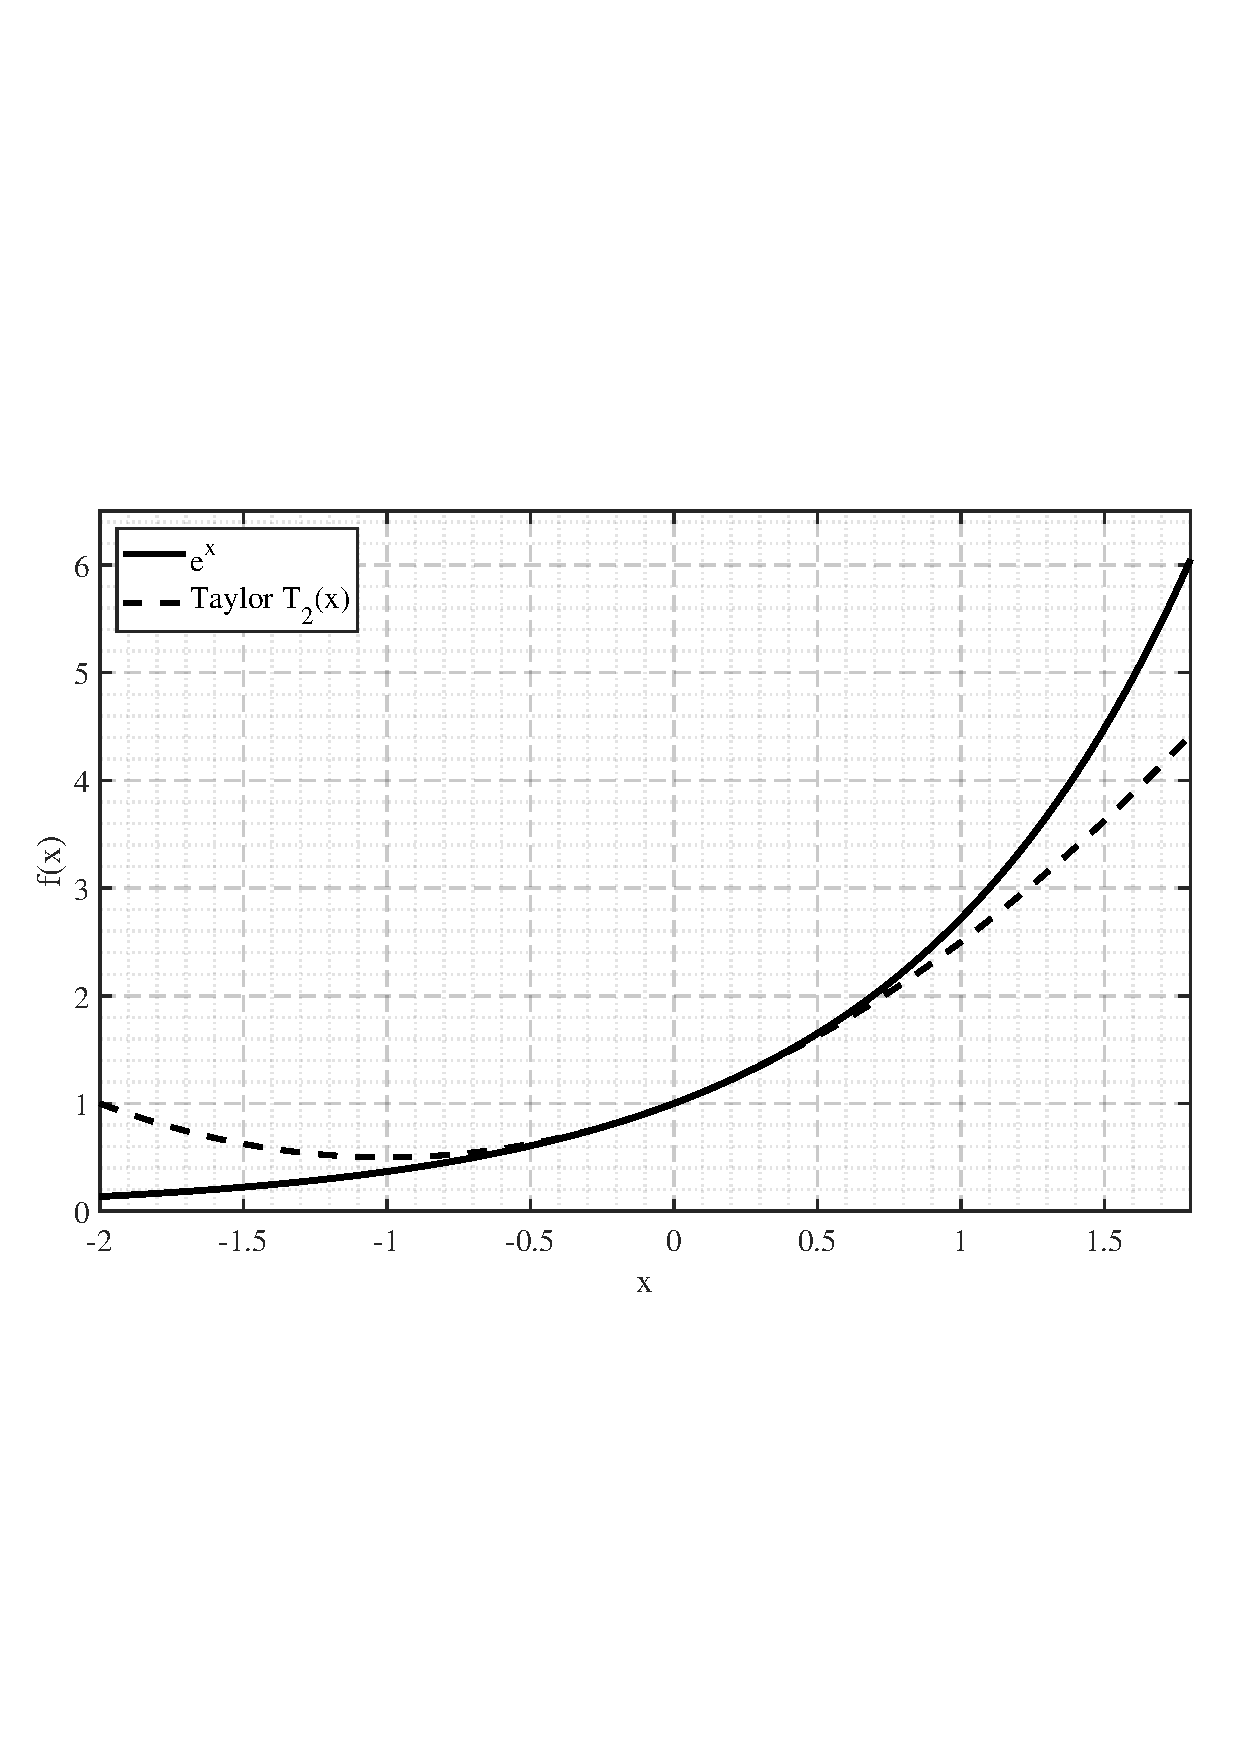
\includegraphics[width=\textwidth]{papers/pade/images/taylorvergleich.pdf}};
\end{tikzpicture}
\caption{TODO
\label{pader:taylorvergleich}}
\end{figure}

Die Ursache hierfür liegt im Aufbau eines Polynoms. Ein Polynom besteht ausschliesslich aus Potenzen der Variablen und besitzt deshalb nur eine begrenzte Flexibilität. Eigenschaften wie starkes exponentielles Wachstum oder asymptotisches Verhalten lassen sich damit nur eingeschränkt beschreiben.

Dies führt zur zentralen Fragestellung dieses Kapitels: Kann dieselbe Information der Taylor-Reihe auf eine andere Weise genutzt werden, um eine genauere Approximation zu erhalten? Genau an dieser Stelle setzt die Padé-Approximation an. Anstatt die Koeffizienten der Taylor-Reihe direkt zu einem Polynom zusammenzufassen, werden sie verwendet, um den Zähler und den Nenner einer rationalen Funktion zu bestimmen. Dadurch entsteht häufig eine deutlich genauere Näherung der ursprünglichen Funktion.

Im nächsten Abschnitt wird dieses Verfahren vorgestellt und anhand der Exponentialfunktion Schritt für Schritt hergeleitet.
